\chapter{Dinâmica do citoesqueleto e motilidade celular}\label{ch:b3:cytoskeleton-motility}

Um neutrófilo que persegue uma bactéria por um tecido rasteja a dez
micrômetros por minuto, mudando de direção em segundos quando o cheiro
se desloca. Uma vesícula de neurotransmissor feita no corpo celular de
um neurônio motor viaja um metro axônio abaixo até o pé, puxada por uma
proteína motora que dá passos de oito nanômetros, cem por segundo,
durante quinze dias. Os \omterm{def:b3:cytoskeleton-motility:cilia}{cílios} que revestem a traqueia batem doze vezes
por segundo em ondas coordenadas que levam à garganta a poeira inalada
de um dia. Tudo isso é feito por três tipos de filamento proteico que
se montam e se desmontam em segundos, e por motores que queimam uma
molécula de ATP por passo. O citoesqueleto não é um esqueleto no
sentido de um arcabouço fixo; é um conjunto de polímeros em renovação
constante, cuja dinâmica \emph{é} o mecanismo da forma, da divisão e do
movimento. Este capítulo trata dos polímeros e de sua cinética, dos
motores e da física que os limita, do rastejamento de uma célula e do
batimento de \omterm{def:b3:cytoskeleton-motility:cilia}{cílios} e flagelos.

\section{Três polímeros}

\begin{definition}[Filamentos de actina, microtúbulos, filamentos intermediários]\label{def:b3:cytoskeleton-motility:filaments}
\index{filamento de actina}\index{microtúbulo}\index{filamento intermediário}\index{polaridade!dos filamentos}\index{centrossomo}
Um \emph{filamento de actina} é um polímero helicoidal de duas fitas de
actina globular, com \qty{7}{nm} de espessura, cada subunidade
ocupando \qty{2.7}{nm} ao longo do eixo, polar: a extremidade
\emph{farpada} (mais) cresce mais depressa que a extremidade
\emph{pontiaguda} (menos), e cada subunidade carrega um ATP que é
hidrolisado depois da incorporação. Um \emph{microtúbulo} é um tubo oco
de \qty{25}{nm} de diâmetro externo, construído com treze
protofilamentos de dímeros de $\alpha\beta$-tubulina (\qty{8}{nm} por
dímero), também polar, com sua extremidade \emph{mais} crescendo mais
depressa e sua extremidade \emph{menos} em geral ancorada no
\emph{centrossomo} perto do núcleo; a subunidade $\beta$ hidrolisa seu
GTP depois da incorporação. Um \emph{filamento intermediário} é uma
corda de \qty{10}{nm} feita de proteínas em hélice enrolada (queratinas
nos epitélios, vimentina no mesênquima, neurofilamentos nos axônios,
lâminas sob o envoltório nuclear), apolar, sem nucleotídeo e bem mais
estável --- um cabo que suporta tensão, e não um trilho dinâmico. A
actina fica sobretudo sob a membrana plasmática e nas protrusões; os
microtúbulos irradiam do centrossomo e servem de trilhos do transporte
de longa distância e de fuso; os filamentos intermediários dão a uma
célula e a seu núcleo sua resiliência mecânica.
\end{definition}

\begin{omfigure}
\begin{tikzpicture}[every node/.style={font=\scriptsize}, >=stealth]
  % actin
  \begin{scope}
    \foreach \i in {0,...,11} { \fill[omThm!70] ({\i*0.4},{0.12*sin(\i*60)}) circle (0.17); }
    \node[below, align=center] at (2.2,-0.5) {filamento de actina, \qty{7}{nm}\\hélice de duas fitas, actina-ATP\\subunidade de \qty{2.7}{nm} ao longo do eixo};
    \node[left] at (-0.3,0) {$-$ pontiaguda}; \node[right] at (4.6,0) {farpada $+$};
  \end{scope}
  % microtubule
  \begin{scope}[xshift=7.2cm]
    \draw[thick, fill=omDef!25] (0,-0.55) rectangle (4.4,0.55);
    \foreach \y in {-0.35,-0.15,0.05,0.25} \draw[omDef] (0,\y) -- (4.4,\y);
    \foreach \x in {0.4,0.8,...,4.0} \draw[omDef] (\x,-0.55) -- (\x,0.55);
    \draw[thick] (4.4,0) ellipse (0.18 and 0.55); \draw[thick, fill=white] (4.4,0) ellipse (0.09 and 0.38);
    \node[below, align=center] at (2.2,-0.65) {microtúbulo, \qty{25}{nm}\\13 protofilamentos de $\alpha\beta$-tubulina (GTP)\\dímero de \qty{8}{nm}};
    \node[left] at (-0.2,0) {$-$}; \node[right] at (4.7,0) {$+$};
  \end{scope}
  % intermediate filament
  \begin{scope}[yshift=-2.9cm, xshift=3.6cm]
    \foreach \dd in {-0.12,0,0.12} \draw[omMeth!70!black, thick] plot[domain=0:4.4, samples=60] (\x, {\dd + 0.1*sin(\x*200 + \dd*400)});
    \node[below, align=center] at (2.2,-0.4) {filamento intermediário, \qty{10}{nm}\\corda em hélice enrolada (queratina, vimentina, lâmina), sem polaridade, sem nucleotídeo};
  \end{scope}
\end{tikzpicture}

{\small Os três filamentos em escala de diâmetro. Os polímeros de
actina e de tubulina são polares e hidrolisam um nucleotídeo depois da
montagem, que é o que os torna dinâmicos; o \omterm{def:b3:cytoskeleton-motility:filaments}{filamento intermediário} é
uma corda apolar feita para durar.}
\end{omfigure}

\begin{omfigure}
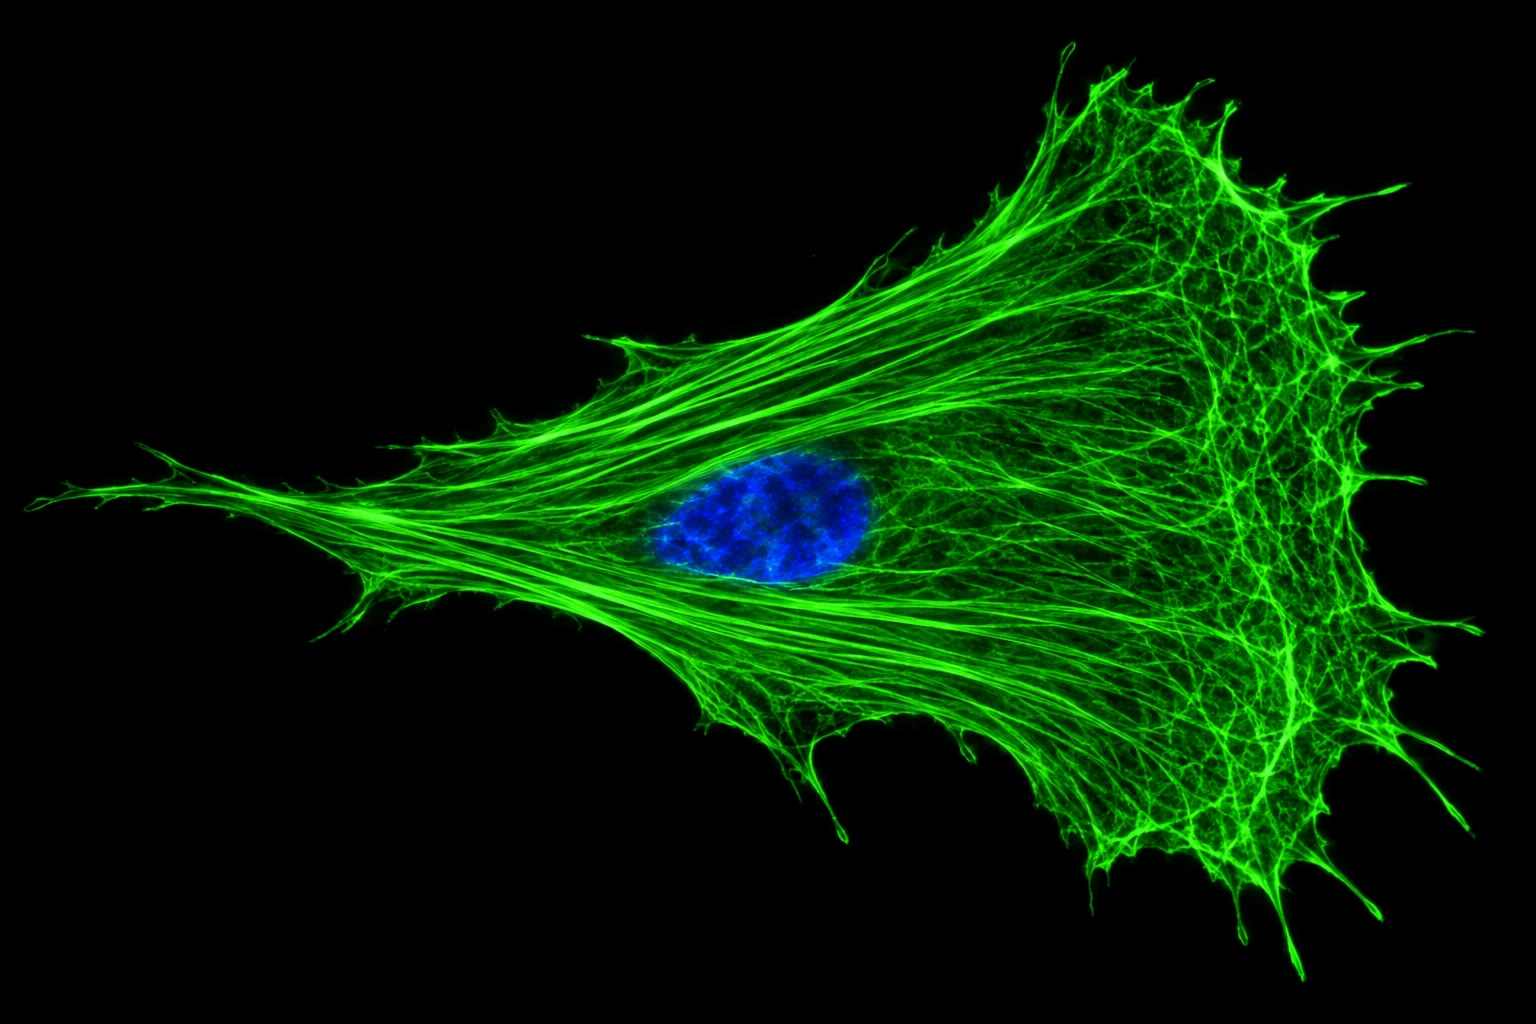
\includegraphics[width=0.54\linewidth]{images/book5/ai/b5-09-fibroblast-actin.jpg}\hspace{0.03\linewidth}
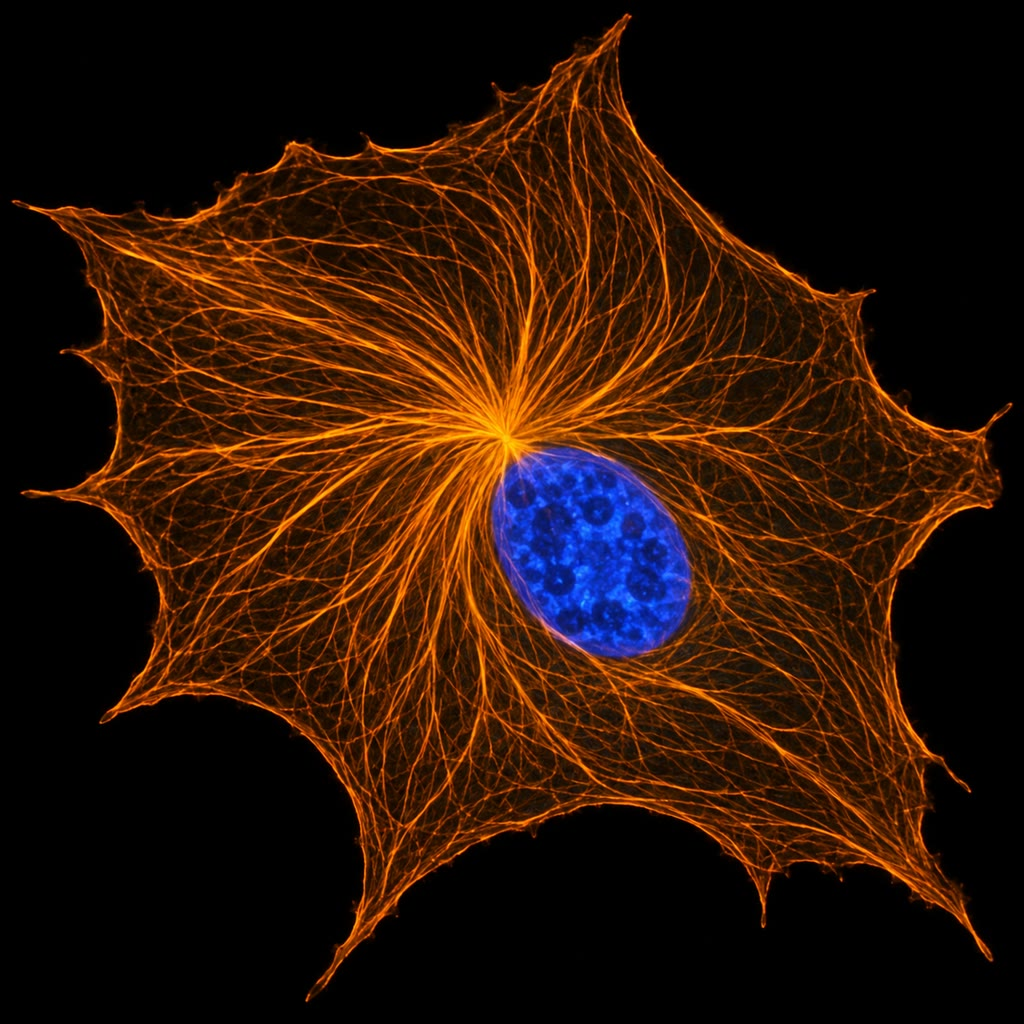
\includegraphics[width=0.36\linewidth]{images/book5/ai/b5-09-microtubules.jpg}

{\small À esquerda: actina (verde) num fibroblasto em migração --- fibras
de estresse atravessando o corpo, uma malha densa na borda de avanço
larga, à direita. À direita: \omterm{def:b3:cytoskeleton-motility:filaments}{microtúbulos} (laranja) irradiando do
\omterm{def:b3:cytoskeleton-motility:filaments}{centrossomo} ao lado do núcleo (azul) até a margem da célula.}
\end{omfigure}

\section{A cinética de um polímero}

\begin{theorem}[Concentração crítica e treadmilling]\label{thm:b3:cytoskeleton-motility:treadmilling}
\index{concentração crítica}\index{treadmilling}
Seja uma extremidade de filamento que acrescenta subunidades à taxa
$k_{\text{on}}C$, com $C$ a concentração de monômero livre, e as perde
à taxa $k_{\text{off}}$. A extremidade cresce se $C$ excede sua
\emph{\omterm{thm:b3:cytoskeleton-motility:treadmilling}{concentração crítica}} $C_{c} = k_{\text{off}}/k_{\text{on}}$ e
encolhe abaixo dela. Se as duas extremidades têm concentrações críticas
diferentes, $C_{c}^{+}
< C_{c}^{-}$, então, no estado estacionário em
que o filamento nem se alonga nem se encurta, a concentração de
monômero é
\[
C_{\text{ss}} = \frac{k_{\text{off}}^{+} + k_{\text{off}}^{-}}
{k_{\text{on}}^{+} + k_{\text{on}}^{-}},
\qquad C_{c}^{+} < C_{\text{ss}} < C_{c}^{-},
\]
e a extremidade mais cresce enquanto a extremidade menos encolhe à
mesma taxa $J = k_{\text{on}}^{+}C_{\text{ss}} - k_{\text{off}}^{+} > 0$: as subunidades fluem pelo filamento da extremidade mais para a
menos --- o \emph{treadmilling} --- ao custo de um nucleotídeo
hidrolisado por subunidade.
\end{theorem}
\begin{proof}
A taxa líquida numa extremidade é $k_{\text{on}}C - k_{\text{off}}$,
nula em $C_{c}$. Comprimento constante exige que a soma das duas taxas
líquidas se anule, o que dá $C_{\text{ss}}$; ela fica entre as duas
concentrações críticas porque é uma média ponderada delas
($C_{\text{ss}} =
(k_{\text{on}}^{+}C_{c}^{+} + k_{\text{on}}^{-}C_{c}^{-})/(k_{\text{on}}^{+}
+ k_{\text{on}}^{-})$). Acima de $C_{c}^{+}$ a extremidade mais cresce;
abaixo de $C_{c}^{-}$ a extremidade menos encolhe; o fluxo é a taxa
líquida da extremidade mais. Duas extremidades do mesmo polímero
químico teriam a mesma $C_{c}$ (a mesma constante de equilíbrio), de
modo que uma diferença exige que a subunidade mude depois da
incorporação --- a hidrólise do ATP ou do GTP ---, o que faz as
extremidades diferirem e paga pelo fluxo.
\end{proof}

\begin{example}[Actina no tubo de ensaio]\label{ex:b3:cytoskeleton-motility:actin-numbers}
Para a actina-ATP, $k_{\text{on}}^{+} = \qty{11.6}{\micro M^{-1}.s^{-1}}$,
$k_{\text{off}}^{+} = \qty{1.4}{s^{-1}}$ ($C_{c}^{+} = \qty{0.12}{\micro
M}$); $k_{\text{on}}^{-} = \qty{1.3}{\micro M^{-1}.s^{-1}}$,
$k_{\text{off}}^{-} = \qty{0.8}{s^{-1}}$ ($C_{c}^{-} = \qty{0.6}{\micro
M}$). Então $C_{\text{ss}} = 2.2/12.9 = \qty{0.17}{\micro M}$ e
$J =
11.6\times 0.17 - 1.4 = 0.6$ subunidade por segundo:
\qty{1.6}{nm/s}, imperceptível. Numa célula os filamentos fazem
treadmilling cem vezes mais depressa, porque a cofilina corta e retira
a actina-ADP velha das extremidades pontiagudas, a profilina carrega
actina-ATP fresca nas extremidades farpadas, e proteínas de capeamento
decidem quais extremidades farpadas podem crescer: o polímero nu
fornece o mecanismo, os reguladores fornecem a velocidade.
\end{example}

\begin{omfigure}
\begin{tikzpicture}
\begin{axis}[
  width=0.7\linewidth, height=5.6cm,
  axis x line=bottom, axis y line=left,
  xmin=0, xmax=1.0, ymin=-1.6, ymax=4,
  xlabel={actina livre ($\unit{\micro M}$)}, ylabel={taxa líquida (subunidades/s)},
  xlabel style={font=\small, at={(axis description cs:0.5,-0.12)}, anchor=north},
  ylabel style={font=\small},
  tick label style={font=\small}, xtick={0,0.2,0.4,0.6,0.8,1.0}, ytick={-1,0,1,2,3,4},
  clip=false,
]
\addplot[thin, gray, domain=0:1.0, samples=2] {0};
\addplot[very thick, omThm, domain=0:0.46, samples=2] {11.6*x-1.4};
\addplot[very thick, omDef, domain=0:1.0, samples=2] {1.3*x-0.8};
\draw[dashed, gray] (axis cs:0.17,-1.6) -- (axis cs:0.17,4);
\node[font=\scriptsize, omThm, anchor=south east] at (axis cs:0.44,3.1) {extremidade farpada};
\node[font=\scriptsize, omDef, anchor=north west] at (axis cs:0.62,-0.25) {extremidade pontiaguda};
\node[font=\scriptsize, anchor=south west] at (axis cs:0.19,3.5) {$C_{\text{ss}}$};
\fill[omThm] (axis cs:0.12,0) circle (2pt); \node[font=\scriptsize, anchor=north east] at (axis cs:0.11,-0.05) {$C_{c}^{+}$};
\fill[omDef] (axis cs:0.6,0) circle (2pt); \node[font=\scriptsize, anchor=south west] at (axis cs:0.61,0.05) {$C_{c}^{-}$};
\end{axis}
\end{tikzpicture}

{\small Taxa líquida de crescimento de cada extremidade de um \omterm{def:b3:cytoskeleton-motility:filaments}{filamento
de actina} contra o monômero livre, com as constantes de taxa do
exemplo. Entre as duas concentrações críticas a extremidade farpada
cresce e a pontiaguda encolhe; na linha tracejada as duas se cancelam
exatamente e o filamento faz treadmilling.}
\end{omfigure}

\begin{definition}[Instabilidade dinâmica]\label{def:b3:cytoskeleton-motility:instability}
\index{instabilidade dinâmica}\index{capuz de GTP}\index{catástrofe}
Os \omterm{def:b3:cytoskeleton-motility:filaments}{microtúbulos} fazem algo mais estranho que o treadmilling. Uma
extremidade mais em crescimento carrega um \emph{capuz de GTP} de
dímeros recém-acrescentados; atrás dele o GTP é hidrolisado, e a
tubulina-GDP, que prefere uma conformação curva, é mantida reta na rede
sob tensão. Se o capuz se perde --- a extremidade faz uma pausa, ou o
crescimento desacelera ---, os protofilamentos tensionados se descascam
para fora e o \omterm{def:b3:cytoskeleton-motility:filaments}{microtúbulo} encurta a \qty{300}{nm/s}, vinte vezes sua
taxa de crescimento: uma \emph{catástrofe}, que termina quando um
dímero de GTP pousa e um novo capuz se forma (um \emph{resgate}). Numa
mesma população, portanto, alguns \omterm{def:b3:cytoskeleton-motility:filaments}{microtúbulos} crescem enquanto
vizinhos colapsam: é a \emph{instabilidade dinâmica}. Ela permite a uma
célula explorar seu próprio volume com extremidades mais a cada poucos
minutos e reconstruir todo o arranjo quando o \omterm{def:b3:cytoskeleton-motility:filaments}{centrossomo} se move ou a
célula se divide. A célula a ajusta por meio de proteínas que
acompanham extremidades mais, estabilizam (tau, MAP2), cortam
(katanina) ou despolimerizam (cinesina-13) \omterm{def:b3:cytoskeleton-motility:filaments}{microtúbulos}; os fármacos
colchicina e os alcaloides da vinca bloqueiam a montagem e o taxol
bloqueia a desmontagem, todos eles venenos do fuso mitótico usados
contra o câncer.
\end{definition}

\begin{proof}[Evidência]
Mitchison e Kirschner (1984) observaram populações de \omterm{def:b3:cytoskeleton-motility:filaments}{microtúbulos}
crescidos a partir de \omterm{def:b3:cytoskeleton-motility:filaments}{centrossomos} in vitro. Ao diluir a tubulina
abaixo da \omterm{thm:b3:cytoskeleton-motility:treadmilling}{concentração crítica}, esperavam que todos os \omterm{def:b3:cytoskeleton-motility:filaments}{microtúbulos}
encurtassem devagar; em vez disso, o número de \omterm{def:b3:cytoskeleton-motility:filaments}{microtúbulos} caiu
enquanto os sobreviventes continuavam crescendo --- alguns haviam se
desmontado por completo e depressa, outros nem um pouco. \omterm{def:b3:cytoskeleton-motility:filaments}{Microtúbulos}
individuais filmados mais tarde por videomicroscopia alternavam
abruptamente entre fases de crescimento constante e de encurtamento
rápido. O \omterm{def:b3:cytoskeleton-motility:instability}{capuz de GTP} explicava as duas coisas: só as extremidades com
capuz crescem, e a perda do capuz é um evento raro, de tudo ou nada.
\end{proof}

\section{Motores}

\begin{definition}[Proteínas motoras]\label{def:b3:cytoskeleton-motility:motors}
\index{miosina}\index{cinesina}\index{dineína}\index{processividade}
Uma \emph{proteína motora} converte a energia livre da hidrólise do ATP
em movimento dirigido ao longo de um filamento: as \emph{miosinas} ao
longo da actina (a miosina II, o motor muscular e contrátil, rumo à
extremidade farpada; a miosina V, uma carregadora de vesículas de duas
cabeças que dá passos de \qty{36}{nm}), as \emph{cinesinas} ao longo
dos \omterm{def:b3:cytoskeleton-motility:filaments}{microtúbulos} rumo à extremidade mais (a cinesina-1 dá passos de
\qty{8}{nm}, um dímero de tubulina, por ATP, mão sobre mão, a cerca de
\qty{800}{nm/s}) e as \emph{dineínas} rumo à extremidade menos (a
dineína citoplasmática, com sua adaptadora dinactina, arrasta a carga
de volta ao centro da célula; as dineínas axonemais dobram os \omterm{def:b3:cytoskeleton-motility:cilia}{cílios}).
Um motor é \emph{processivo} se dá muitos passos antes de se soltar: a
cinesina-1 caminha cerca de um micrômetro, uma centena de passos,
sozinha; uma única cabeça de miosina II dá uma remada e solta, de modo
que o músculo precisa de centenas de cabeças trabalhando num mesmo
filamento. Os motores leem a polaridade do trilho, e por isso a
geografia de uma célula --- extremidades mais na periferia,
extremidades menos no centro --- é um mapa de aonde cada motor levará
sua carga.
\end{definition}

\begin{proof}[Evidência]
Vale, Reese e Sheetz (1985) descobriram a \omterm{def:b3:cytoskeleton-motility:motors}{cinesina} como a proteína do
axoplasma de lula que fazia esferas de látex deslizarem ao longo de
\omterm{def:b3:cytoskeleton-motility:filaments}{microtúbulos} no sentido mais, e nos anos seguintes a estrutura de duas
cabeças, o sentido de cada família e a parceira retrógrada \omterm{def:b3:cytoskeleton-motility:motors}{dineína}
foram esclarecidos. Svoboda, Schmidt, Schnapp e Block (1993) seguraram
numa pinça óptica uma esfera que carregava uma única \omterm{def:b3:cytoskeleton-motility:motors}{cinesina} e
registraram sua posição com resolução de nanômetros: a esfera avançava
em passos discretos de \qty{8}{nm}, um por ATP em baixa concentração de
ATP, e parava contra uma força de cerca de \qty{6}{pN}. A escada
molecular foi vista diretamente.
\end{proof}

\begin{omfigure}
\begin{tikzpicture}[every node/.style={font=\scriptsize}, >=stealth]
  % left: kinesin on a microtubule
  \begin{scope}
    \draw[thick, fill=omDef!25] (0,0) rectangle (5.4,0.5);
    \foreach \x in {0.4,0.8,...,5.2} \draw[omDef] (\x,0) -- (\x,0.5);
    \node[left] at (-0.1,0.25) {$-$}; \node[right] at (5.5,0.25) {$+$};
    % two heads, stalk, cargo
    \fill[omProp] (2.4,0.72) circle (0.2); \fill[omProp!60] (3.2,0.72) circle (0.2);
    \draw[thick, omProp!80!black] (2.6,0.85) -- (2.85,1.4) -- (3.05,0.85); \draw[thick, omProp!80!black] (2.85,1.4) -- (2.85,2.3);
    \draw[thick, fill=omExo!40] (2.85,2.7) circle (0.4); \node at (2.85,2.7) {carga};
    \draw[->, thick, omThm] (3.4,0.72) arc[start angle=180, end angle=0, radius=0.4] ; \node[right, omThm] at (3.85,1.15) {\qty{8}{nm} por ATP};
    \node[below, align=center] at (2.7,-0.1) {a cinesina-1 caminha mão sobre mão rumo à extremidade mais;\\cerca de $100$ passos por segundo, \qty{0.8}{\micro m/s}};
  \end{scope}
  % right: optical trap staircase
  \begin{scope}[xshift=7.2cm, yshift=-0.6cm]
  \begin{axis}[
    width=5.6cm, height=4.4cm, axis lines=left,
    xmin=0, xmax=1.0, ymin=0, ymax=40,
    xlabel={tempo (s)}, ylabel={posição (nm)},
    xlabel style={font=\scriptsize, at={(axis description cs:0.5,-0.12)}, anchor=north},
    ylabel style={font=\scriptsize},
    tick label style={font=\scriptsize}, xtick={0,0.5,1.0}, ytick={0,8,16,24,32},
  ]
  \addplot[very thick, omProp!80!black, const plot] coordinates {(0,0) (0.18,8) (0.31,16) (0.55,24) (0.71,32) (1.0,32)};
  \end{axis}
  \node[font=\scriptsize, align=center] at (2.8,3.6) {um motor isolado numa pinça óptica,\\ATP baixo: passos de \qty{8}{nm}};
  \end{scope}
\end{tikzpicture}

{\small A \omterm{def:b3:cytoskeleton-motility:motors}{cinesina} em seu trilho e sua pegada numa pinça óptica. As
duas cabeças se alternam, e cada passo avança o motor por um dímero de
tubulina, \qty{8}{nm}; em ATP baixo os passos são separados por esperas
pelo nucleotídeo seguinte e a escada é vista diretamente.}
\end{omfigure}

\begin{proposition}[O que a física permite a um motor]\label{prop:b3:cytoskeleton-motility:physics}
\index{força de parada}\index{energia térmica}\index{difusão contra transporte}
A hidrólise de um ATP na célula libera cerca de \qty{50}{kJ/mol}, isto
é, $8\times 10^{-20}$ J por molécula. Um motor que avança $d$ por ATP
contra uma força $F$ realiza um trabalho $Fd$, de modo que sua
\emph{\omterm{prop:b3:cytoskeleton-motility:physics}{força de parada}} não pode exceder $F_{\max} = \Delta G/d$: para o
passo de \qty{8}{nm} da \omterm{def:b3:cytoskeleton-motility:motors}{cinesina}, \qty{10}{pN}; os \qty{6}{pN} medidos
significam uma eficiência perto de \qty{60}{\%}, maior que a de
qualquer motor térmico. A \omterm{prop:b3:cytoskeleton-motility:physics}{energia térmica} $k_{B}T =
4.1\times 10^{-21}$ J, ou \qty{4.1}{pN.nm}, é apenas um vigésimo da
energia do ATP, mas é entregue ao motor sem parar como chutes
brownianos; um motor é um dispositivo que os retifica, deixando a
cabeça difundir para a frente e ligando-se quando ela pousa, de modo
que a energia química é gasta em tornar o passo irreversível, e não em
empurrar. O transporte por motor vence a difusão em qualquer distância
que importe numa célula grande: uma vesícula com coeficiente de difusão
$D = \qty{1}{\micro
m^2/s}$ precisa de um tempo $L^{2}/2D$ para
vagar uma distância $L$ --- meio segundo para um micrômetro, mas
\num{16000} anos para um metro de axônio ---, ao passo que um motor a
\qty{1}{\micro m/s} cobre o metro em doze dias.
\end{proposition}
\admitted

\section{Como uma célula rasteja}

\begin{definition}[Migração celular]\label{def:b3:cytoskeleton-motility:migration}
\index{lamelipódio}\index{complexo Arp2/3}\index{adesão focal}\index{integrina}\index{GTPases Rho}
Uma célula que rasteja repete um ciclo de quatro etapas. A
\emph{protrusão}: na borda de avanço a actina polimeriza contra a
membrana numa lâmina, o \emph{lamelipódio}, cuja rede ramificada é
construída pelo \emph{complexo Arp2/3}, que nucleia um filamento novo a
partir do flanco de um já existente a \qty{70}{\degree}, enquanto a
proteína de capeamento limita o crescimento de cada filamento e a
cofilina recicla a rede alguns micrômetros atrás; \emph{filopódios} em
forma de dedo, de filamentos em feixe, sondam à frente. A
\emph{adesão}: a nova protrusão se prende ao substrato por meio das
\emph{integrinas}, receptores transmembrana que ligam proteínas da
matriz do lado de fora e, por meio de proteínas adaptadoras, a actina
do lado de dentro, agrupadas em \emph{adesões focais}. A
\emph{contração}: a \omterm{def:b3:cytoskeleton-motility:motors}{miosina} II puxa as fibras de estresse ancoradas nas
adesões, arrastando o corpo celular para a frente. A \emph{retração}:
as adesões da retaguarda se soltam e a cauda é recolhida. O ciclo é
coordenado por três \omterm{def:b3:membrane-traffic:coats}{GTPases pequenas} da família \emph{Rho} --- a Rac
impulsiona os lamelipódios, a Cdc42 os filopódios, a Rho as fibras de
estresse e a contração ---, que são os alvos dos receptores que leem a
direção de um gradiente químico (quimiotaxia) ou a rigidez e o padrão
do substrato.
\end{definition}

\begin{omfigure}
\begin{tikzpicture}[every node/.style={font=\scriptsize}, >=stealth]
  % substrate
  \draw[very thick, gray] (0,0) -- (12,0); \node[below right, gray] at (0,-0.05) {substrato (matriz)};
  % cell outline
  \draw[thick, omDef, fill=omDef!10] (1.0,0.05) .. controls (1.2,1.4) and (3.0,2.3) .. (5.0,2.2) .. controls (7.0,2.1) and (8.6,1.4) .. (9.8,0.6) .. controls (10.3,0.4) and (10.8,0.2) .. (11.2,0.05) -- cycle;
  % nucleus
  \draw[thick, fill=omDef!40] (4.6,1.1) ellipse (1.0 and 0.6); \node at (4.6,1.1) {núcleo};
  % lamellipodium: branched actin
  \foreach \p/\a in {(9.9,0.3)/20,(10.1,0.5)/-10,(10.3,0.25)/35,(10.6,0.45)/5,(10.4,0.7)/-25,(9.7,0.7)/15} { \draw[omThm, thick] \p -- ++(\a:0.55); \draw[omThm, thick] \p ++(\a:0.3) -- ++(\a+70:0.35); }
  \node[right, align=left, omThm] at (11.3,1.3) {1. protrusão:\\actina ramificada pelo Arp2/3\\empurra a membrana};
  \draw[->, thick, omThm] (11.3,0.3) -- (11.9,0.3);
  % focal adhesions
  \foreach \x in {9.3,7.6,2.4} \fill[omProp] (\x-0.25,0.03) rectangle (\x+0.25,0.18);
  \node[below, omProp, align=center] at (9.3,-0.45) {2. adesão: integrinas,\\adesões focais};
  % stress fibres and myosin
  \foreach \y in {0.45,0.75} \draw[omMeth!70!black, thick] (2.5,\y) -- (7.5,\y+0.1);
  \node[above, omMeth!70!black, align=center] at (7.8,2.3) {3. contração: miosina II\\nas fibras de estresse};
  \draw[->, thick, omMeth!70!black] (6.0,1.55) -- (6.8,1.55);
  % retraction at rear
  \draw[->, thick, gray] (0.8,0.9) -- (1.6,0.9); \node[above, align=center] at (1.4,2.35) {4. retração:\\as adesões traseiras se soltam};
\end{tikzpicture}

{\small O ciclo do rastejamento, com o sentido da esquerda para a
direita como o do deslocamento: a polimerização ramificada de actina
empurra a frente para fora, as \omterm{def:b3:cytoskeleton-motility:migration}{integrinas} a ancoram, a \omterm{def:b3:cytoskeleton-motility:motors}{miosina} puxa o
corpo para a frente, e a retaguarda se solta.}
\end{omfigure}

\begin{example}[O cometa da Listeria]\label{ex:b3:cytoskeleton-motility:listeria}
A bactéria \emph{Listeria monocytogenes}, uma vez dentro de uma célula,
exibe em sua superfície uma única proteína, a ActA, que recruta o
\omterm{def:b3:cytoskeleton-motility:migration}{complexo Arp2/3} do hospedeiro. A actina polimeriza na superfície
bacteriana e fica para trás como uma cauda; a bactéria é empurrada pelo
citoplasma a até \qty{0.5}{\micro m/s} e para dentro das células
vizinhas sem jamais deixar o citosol. A cauda é um \omterm{def:b3:cytoskeleton-motility:migration}{lamelipódio} virado
do avesso, com uma proteína onde a célula usa dezenas, e mostrou que a
polimerização da actina sozinha --- sem motor algum --- gera a força da
protrusão: cada subunidade que se insere entre a rede e a membrana,
quando uma flutuação térmica abriu uma fresta, empurra a frente
\qty{2.7}{nm} adiante como uma catraca.
\end{example}

\begin{method}[Observar a renovação dos polímeros]\label{met:b3:cytoskeleton-motility:frap}
\index{recuperação de fluorescência após fotobranqueamento}\index{microscopia de speckles}
Para medir a dinâmica de um sistema de filamentos numa célula viva: (1)
expresse a subunidade fundida a uma proteína fluorescente em nível
baixo, de modo que ela seja incorporada ao polímero endógeno; (2) ou
branqueie uma pequena região com um pulso intenso de laser e filme o
retorno da fluorescência à medida que subunidades não branqueadas
entram por troca (\emph{\omterm{met:b3:cytoskeleton-motility:frap}{recuperação de fluorescência após
fotobranqueamento}}, FRAP) --- o tempo de meia-recuperação é o tempo de
residência das subunidades, e a fração que nunca se recupera é a
reserva imóvel; ou (3) expresse tão pouca subunidade marcada que o
polímero apareça como \emph{speckles} esparsos, e rastreie-os: seu
movimento é o fluxo do treadmilling, e seu surgimento e desaparecimento
são a montagem e a desmontagem. Num \omterm{def:b3:cytoskeleton-motility:migration}{lamelipódio} os speckles fluem para
trás a um micrômetro por minuto em relação ao substrato enquanto a
borda avança: a rede é construída na frente e consumida alguns
micrômetros atrás dela.
\end{method}

\section{Cílios, flagelos e um motor rotativo}

\begin{definition}[Cílios e flagelos]\label{def:b3:cytoskeleton-motility:cilia}
\index{cílio}\index{axonema}\index{dineína axonemal}\index{cílio primário}\index{transporte intraflagelar}
Um \emph{cílio} ou \emph{flagelo} eucarionte é uma extensão recoberta de
membrana construída sobre o \emph{axonema}: nove \omterm{def:b3:cytoskeleton-motility:filaments}{microtúbulos} duplos em
anel em torno de um par central, mantidos por ligações de nexina e
raios radiais, e crescidos a partir de um corpúsculo basal, um
centríolo modificado. As \emph{\omterm{def:b3:cytoskeleton-motility:motors}{dineínas} axonemais} presas a cada duplo
caminham ao longo do duplo vizinho rumo à extremidade menos dele, na
base; como os duplos estão amarrados uns aos outros, eles não podem
deslizar livremente, e o deslizamento é convertido em dobramento,
propagado ao longo do axonema como uma onda pela alternância das
\omterm{def:b3:cytoskeleton-motility:motors}{dineínas} ativas de um lado do anel para o outro. Um cílio tem de
\qtyrange{5}{10}{\micro m} de comprimento e bate de \numrange{10}{20}
vezes por segundo; um flagelo de espermatozoide tem \qty{50}{\micro m}
e ondula. As proteínas de um cílio são levadas do corpo celular para
cima pela cinesina-2 e de volta pela dineína-2 ao longo dos duplos ---
o \emph{transporte intraflagelar} ---, que é também como se constrói um
\emph{cílio primário} não móvel, presente, um por célula, na maioria
das células de vertebrado; esse cílio é uma antena sensorial, que
abriga receptores para a luz (o segmento externo do bastonete),
odores, fluxo e sinais do desenvolvimento, e cujos defeitos causam as
\emph{ciliopatias}: rins policísticos, degeneração da retina, obesidade,
dedos extras.
\end{definition}

\begin{omfigure}
\begin{tikzpicture}[every node/.style={font=\scriptsize}, >=stealth]
  % axoneme cross-section
  \begin{scope}
    \draw[thick, omDef!60] (0,0) circle (1.75);
    \foreach \i in {0,...,8} { \begin{scope}[rotate=\i*40] \draw[thick, fill=omDef!30] (0,1.3) circle (0.16); \draw[thick, fill=omDef!30] (0.27,1.22) circle (0.13); \draw[omProp, thick] (0.15,1.05) -- (0.05,0.5); \draw[omThm, thick] (0.4,1.28) -- (0.62,1.2); \end{scope} }
    \draw[thick, fill=omDef!30] (-0.15,0) circle (0.16); \draw[thick, fill=omDef!30] (0.15,0) circle (0.16);
    \node[right, align=left] at (2.0,1.2) {9 microtúbulos duplos}; \draw (1.9,1.2) -- (1.35,1.0);
    \node[right, align=left] at (2.0,0.4) {par central}; \draw (1.9,0.4) -- (0.35,0.1);
    \node[right, align=left, omThm] at (2.0,-0.4) {os braços de dineína de cada\\duplo alcançam o seguinte}; \draw[omThm] (1.9,-0.3) -- (1.0,-0.85);
    \node[right, align=left, omProp] at (2.0,-1.3) {raios radiais}; \draw[omProp] (1.9,-1.3) -- (0.4,-0.7);
    \node[below] at (0,-1.9) {axonema, \qty{0.25}{\micro m} de diâmetro};
  \end{scope}
  % bending from sliding
  \begin{scope}[xshift=7.6cm]
    \draw[very thick, omDef] (0,-1.6) -- (0,1.6); \draw[very thick, omDef] (0.5,-1.6) -- (0.5,1.6);
    \draw[->, thick, omThm] (0.1,0.5) -- (0.4,0.5); \draw[->, thick, omThm] (0.1,-0.2) -- (0.4,-0.2);
    \node[below, align=center] at (0.25,-1.7) {as dineínas de um duplo\\empurram o vizinho\\rumo à ponta};
    \draw[->, thick] (1.5,0) -- (2.5,0);
    \draw[very thick, omDef] (3.6,-1.6) .. controls (3.6,-0.3) and (4.6,0.5) .. (4.4,1.6); \draw[very thick, omDef] (4.1,-1.6) .. controls (4.1,-0.3) and (5.1,0.5) .. (4.9,1.6);
    \node[below, align=center] at (4.3,-1.7) {amarrados na base e pela nexina,\\os duplos não podem deslizar:\\eles se dobram};
  \end{scope}
\end{tikzpicture}

{\small O \omterm{def:b3:cytoskeleton-motility:cilia}{axonema} em corte transversal (à esquerda): nove duplos em
torno de um par central, com braços de \omterm{def:b3:cytoskeleton-motility:motors}{dineína} e raios radiais. À
direita: as \omterm{def:b3:cytoskeleton-motility:motors}{dineínas} deslizam um duplo ao longo do seguinte e, como os
duplos estão amarrados, o deslizamento vira um dobramento que viaja ao
longo do \omterm{def:b3:cytoskeleton-motility:cilia}{cílio}.}
\end{omfigure}

\begin{omfigure}
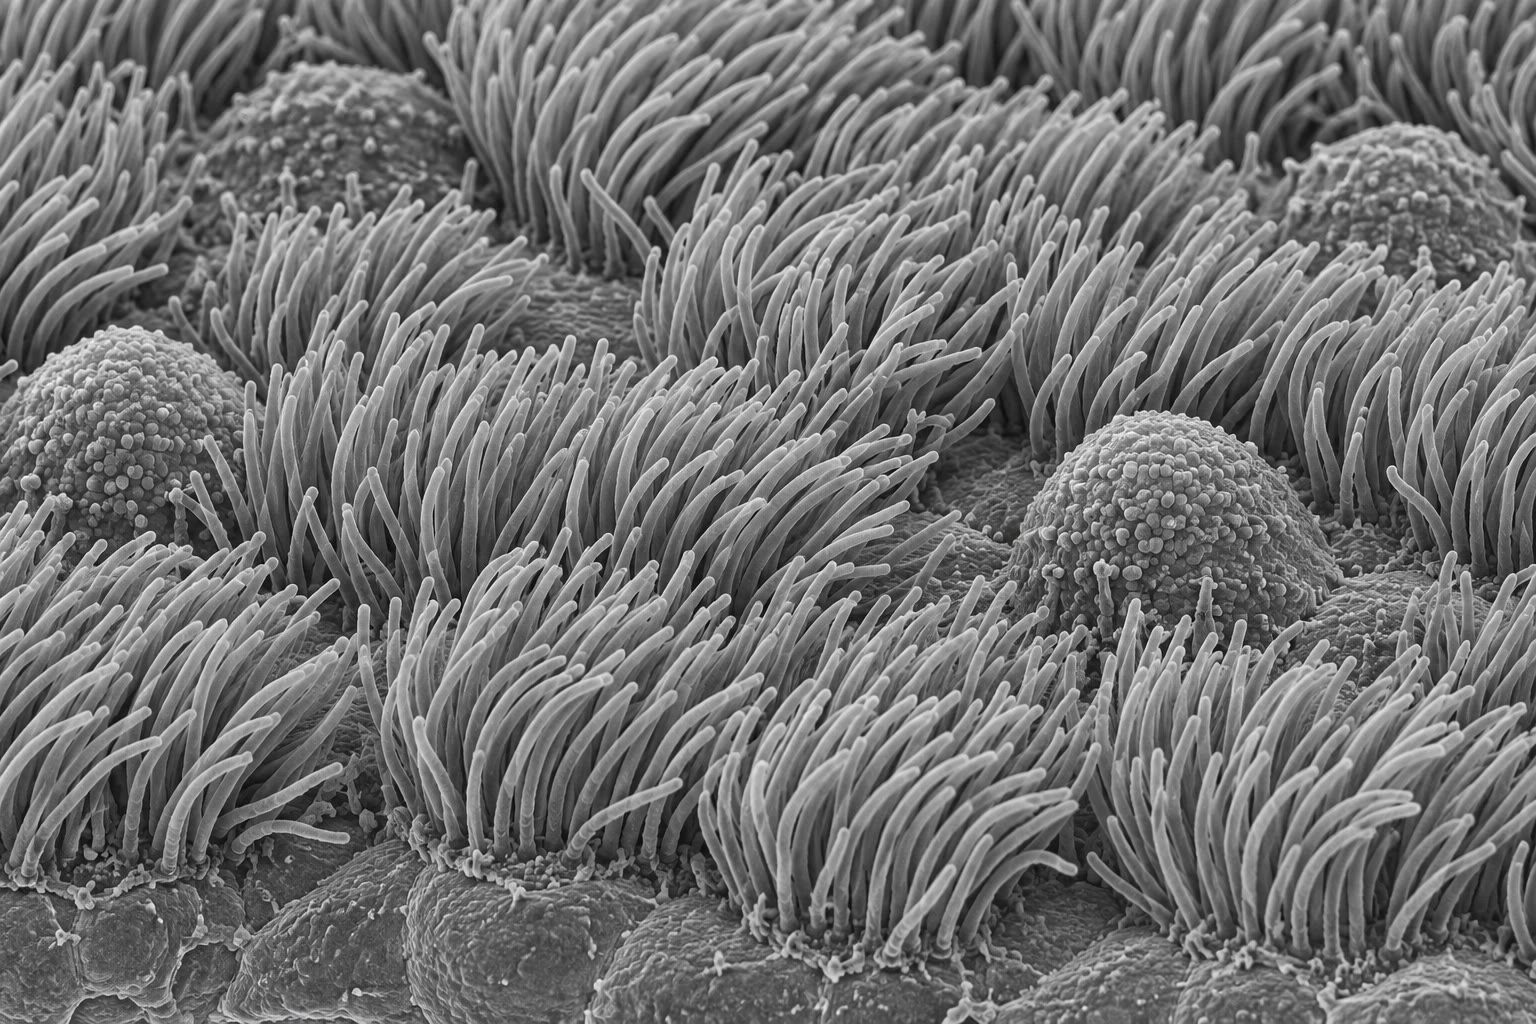
\includegraphics[width=0.54\linewidth]{images/book5/ai/b5-09-cilia-sem.jpg}\hspace{0.03\linewidth}
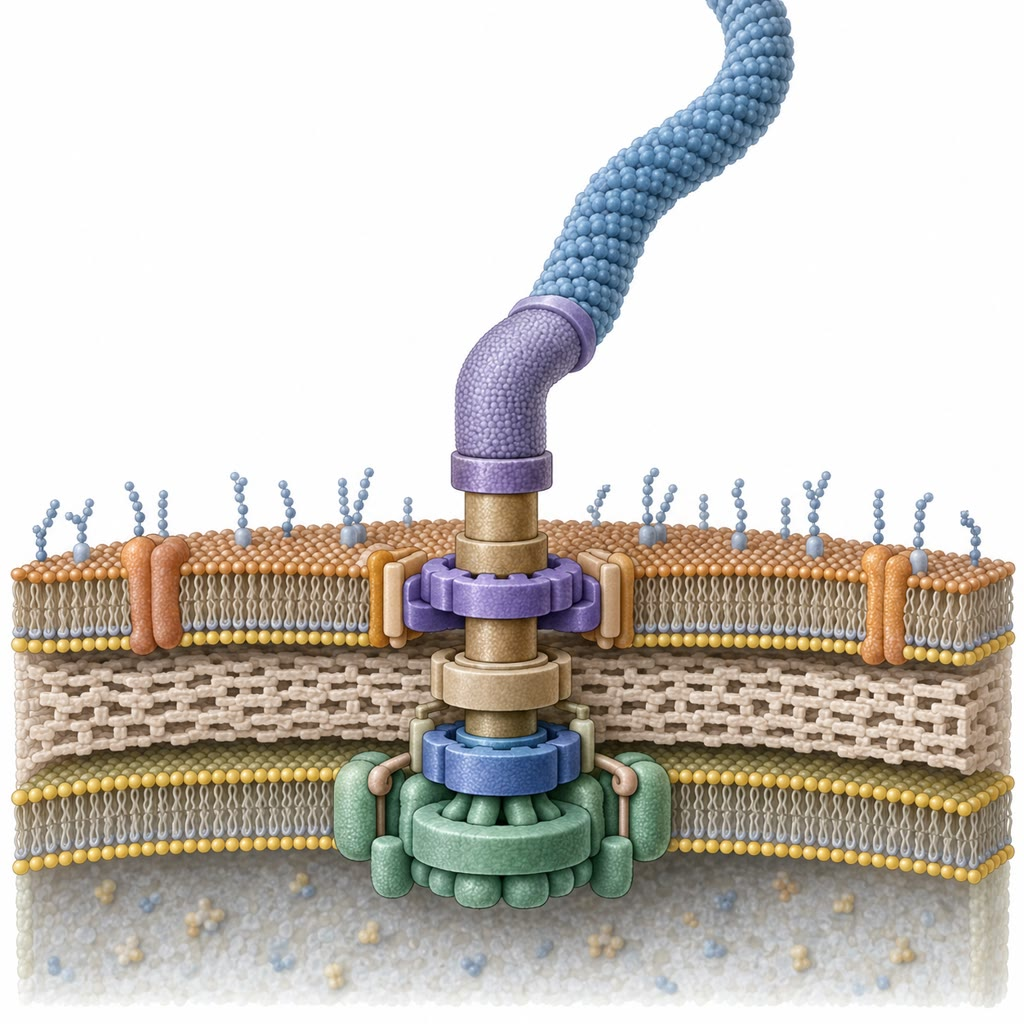
\includegraphics[width=0.36\linewidth]{images/book5/ai/b5-09-flagellar-motor.jpg}

{\small À esquerda: o epitélio ciliado da traqueia no microscópio
eletrônico de varredura, um gramado de \omterm{def:b3:cytoskeleton-motility:cilia}{cílios} entre células secretoras
de muco em forma de cúpula. À direita: o \omterm{prop:b3:cytoskeleton-motility:flagellar-motor}{motor flagelar} bacteriano, um
motor rotativo de anéis no envoltório celular movido pelo fluxo de
prótons.}
\end{omfigure}

\begin{proposition}[O motor flagelar bacteriano]\label{prop:b3:cytoskeleton-motility:flagellar-motor}
\index{motor flagelar}\index{corrida e tombo}
O flagelo bacteriano não tem parentesco com o eucarionte: um filamento
helicoidal rígido de flagelina, de \qty{20}{nm} de espessura e vários
micrômetros de comprimento, girado por um \emph{motor rotativo}
embutido no envoltório celular --- um rotor de umas quarenta e cinco
proteínas cercado por um anel de unidades estatoras, cada uma um canal
pelo qual os prótons fluem gradiente abaixo para dentro da célula,
cerca de mil prótons por volta. O motor gira a até \qty{300}{Hz},
inverte o sentido em um milissegundo e desenvolve um torque de uns
\qty{1000}{pN.nm}; é construído com umas vinte proteínas cujos genes
são ligados na ordem em que as peças são montadas, de dentro para fora.
Em \emph{E.~coli}, a rotação anti-horária reúne os vários flagelos num
propulsor e a célula \emph{corre} em linha reta; uma troca para o
sentido horário desfaz o feixe e a célula \emph{tomba} rumo a uma nova
direção aleatória. A via de quimiotaxia não enviesa nada além da
frequência dos tombos --- menos quando as condições melhoram --- e isso
basta para subir um gradiente.
\end{proposition}

\begin{remark}[O citoesqueleto é um verbo]\label{rem:b3:cytoskeleton-motility:verb}
Quase nada do que se descreveu neste capítulo é uma estrutura no
sentido em que um osso é: o \omterm{def:b3:cytoskeleton-motility:migration}{lamelipódio} é uma onda de polimerização, o
fuso do \cref{ch:b3:cell-cycle-apoptosis} é um estado estacionário de
\omterm{def:b3:cytoskeleton-motility:filaments}{microtúbulos} que crescem e colapsam, o batimento do \omterm{def:b3:cytoskeleton-motility:cilia}{cílio} é um padrão
de alternância de motores. A renovação não é um custo que a célula
tolera, mas o próprio mecanismo, e é por isso que cada um desses
sistemas funciona à base de hidrólise de nucleotídeo e para em minutos
quando o ATP se esgota, e por isso que os venenos que congelam os
polímeros num estado ou no outro --- taxol ou colchicina, faloidina ou
citocalasina --- são igualmente letais.
\end{remark}

\section{Exercícios}

\begin{exercise}[$\star$]\label{exo:b3:cytoskeleton-motility:1}
Compare os \omterm{def:b3:cytoskeleton-motility:filaments}{filamentos de actina}, os \omterm{def:b3:cytoskeleton-motility:filaments}{microtúbulos} e os \omterm{def:b3:cytoskeleton-motility:filaments}{filamentos
intermediários} quanto a diâmetro, subunidade, polaridade, nucleotídeo e
papel típico.
\end{exercise}

\begin{exercise}[$\star$]\label{exo:b3:cytoskeleton-motility:2}
Defina \omterm{thm:b3:cytoskeleton-motility:treadmilling}{concentração crítica}. Por que as duas extremidades de um
\omterm{def:b3:cytoskeleton-motility:filaments}{filamento de actina} têm concentrações críticas diferentes, e o que
aconteceria se elas fossem iguais?
\end{exercise}

\begin{exercise}[$\star$]\label{exo:b3:cytoskeleton-motility:3}
Nomeie um motor para cada caso: vesícula rumo à periferia da célula
sobre \omterm{def:b3:cytoskeleton-motility:filaments}{microtúbulos}; vesícula rumo ao centro; contração de uma fibra de
estresse; dobramento de um \omterm{def:b3:cytoskeleton-motility:cilia}{cílio}. Dê o sentido que cada um toma em seu
trilho.
\end{exercise}

\begin{exercise}[$\star$]\label{exo:b3:cytoskeleton-motility:4}
Liste as quatro etapas do ciclo de rastejamento e a GTPase da família
Rho que governa cada uma das três primeiras.
\end{exercise}

\begin{exercise}[$\star\star$]\label{exo:b3:cytoskeleton-motility:5}
A extremidade mais de um polímero tem
$k_{\text{on}} = \qty{5}{\micro M^{-1}.s^{-1}}$,
$k_{\text{off}} = \qty{1}{s^{-1}}$, e sua extremidade menos
$k_{\text{on}} =
\qty{1}{\micro M^{-1}.s^{-1}}$,
$k_{\text{off}} = \qty{0.8}{s^{-1}}$. Determine as duas concentrações
críticas, a concentração estacionária e a taxa de treadmilling em
subunidades por segundo e, para subunidades de \qty{2.7}{nm}, em
nanômetros por segundo.
\end{exercise}

\begin{exercise}[$\star\star$]\label{exo:b3:cytoskeleton-motility:6}
A \omterm{def:b3:cytoskeleton-motility:motors}{cinesina} caminha a \qty{800}{nm/s} com passos de \qty{8}{nm}, um ATP
cada. Quantos ATP por segundo por motor? O axônio de um neurônio tem
\qty{1}{m}: quanto dura a viagem, e quantos ATP um motor gasta nela?
Compare com o tempo de difusão da
\cref{prop:b3:cytoskeleton-motility:physics}.
\end{exercise}

\begin{exercise}[$\star\star$]\label{exo:b3:cytoskeleton-motility:7}
A \omterm{def:b3:cytoskeleton-motility:motors}{miosina} V dá passos de \qty{36}{nm} por ATP. Qual é sua \omterm{prop:b3:cytoskeleton-motility:physics}{força de
parada} máxima, e por que ela é menor que a da \omterm{def:b3:cytoskeleton-motility:motors}{cinesina}? Qual motor é
mais adequado a carregar uma carga grande, e qual a mover-se depressa?
\end{exercise}

\begin{exercise}[$\star\star$]\label{exo:b3:cytoskeleton-motility:8}
Preveja o efeito sobre uma célula em divisão, e sobre uma célula que
rasteja, de (a) taxol, (b) colchicina, (c) citocalasina, (d) um
inibidor de Rac, e explique cada um pelo mecanismo.
\end{exercise}

\begin{exercise}[$\star\star$]\label{exo:b3:cytoskeleton-motility:9}
Num experimento de FRAP num \omterm{def:b3:cytoskeleton-motility:migration}{lamelipódio}, a fluorescência se recupera
com meia-recuperação de \qty{20}{s} até \qty{90}{\%} de seu valor
inicial. Quais são o tempo de residência da actina na rede e a fração
imóvel? Os speckles fluem para trás a \qty{1.5}{\micro m/min} enquanto
a borda avança a \qty{1}{\micro m/min}: a que taxa a actina está
polimerizando na borda?
\end{exercise}

\begin{exercise}[$\star\star\star$]\label{exo:b3:cytoskeleton-motility:10}
Explique a \omterm{def:b3:cytoskeleton-motility:instability}{instabilidade dinâmica} em termos do \omterm{def:b3:cytoskeleton-motility:instability}{capuz de GTP} e mostre
por que uma população de \omterm{def:b3:cytoskeleton-motility:filaments}{microtúbulos} mantida logo acima da
\omterm{thm:b3:cytoskeleton-motility:treadmilling}{concentração crítica} se torna bimodal em comprimento, em vez de
uniforme. O que a célula ganha com um comportamento que desperdiça GTP?
\end{exercise}

\begin{exercise}[$\star\star\star$]\label{exo:b3:cytoskeleton-motility:11}
Uma bactéria de \qty{2}{\micro m} nada a \qty{25}{\micro m/s}. Na água,
nessa escala, o arrasto viscoso domina e a célula para dentro de um
nanômetro quando o motor para. Explique por que um movimento recíproco
(um remo) não consegue propulsioná-la e uma hélice em rotação consegue,
e estime o número de prótons que o motor gasta por segundo a
\qty{100}{Hz}.
\end{exercise}

\begin{exercise}[$\star\star\star$]\label{exo:b3:cytoskeleton-motility:12}
A síndrome de Kartagener --- \omterm{def:b3:cytoskeleton-motility:cilia}{cílios} imóveis --- dá bronquite crônica,
infertilidade masculina e, em metade dos pacientes, um coração do lado
direito. Explique cada uma dessas coisas pela biologia do \omterm{def:b3:cytoskeleton-motility:cilia}{axonema}, e
diga por que a última afeta apenas metade.
\end{exercise}

\section{Problema: um neutrófilo em movimento}

\begin{problem}[{Problema de fim de semana --- o orçamento de actina de
um neutrófilo contado, seu treadmilling calculado, a viagem de uma
vesícula axônio abaixo cronometrada contra a difusão, a eficiência de
um motor medida e a polimerização e o custo em ATP da frente de
rastejamento resolvidos, terminando na taxa de treadmilling, no tempo
para atravessar um axônio e no ATP que um lamelipódio queima por
segundo}]
\label{pb:b3:cytoskeleton-motility:1}
Dados: um neutrófilo de volume \qty{300}{\micro m^3} contém actina a
\qty{200}{\micro M}, metade polimerizada; uma subunidade acrescenta
\qty{2.7}{nm} a um filamento. Constantes de taxa da actina como no
\cref{ex:b3:cytoskeleton-motility:actin-numbers}. \omterm{def:b3:cytoskeleton-motility:motors}{Cinesina}: passos de
\qty{8}{nm}, \qty{800}{nm/s}, \omterm{prop:b3:cytoskeleton-motility:physics}{força de parada} \qty{6}{pN}; hidrólise do
ATP $\Delta G = \qty{50}{kJ/mol}$; $k_{B}T = \qty{4.1}{pN.nm}$;
coeficiente de difusão da vesícula \qty{1}{\micro m^2/s}; comprimento
do axônio \qty{1}{m}. O \omterm{def:b3:cytoskeleton-motility:migration}{lamelipódio} tem \qty{20}{\micro m} de largura
com $200$ filamentos por micrômetro de borda, avançando a
\qty{10}{\micro m/min}; a rede é desmontada \qty{3}{\micro m} atrás da
borda.

\medskip
\noindent\textbf{Parte I --- O orçamento de actina.}
\begin{enumerate}
  \item Quantas moléculas de actina a célula contém, e quantas estão em
        filamentos?
  \item Que comprimento total de filamento é esse? Se o filamento médio
        tem \qty{0.25}{\micro m}, quantos filamentos?
  \item A actina livre está a \qty{100}{\micro M}, muito acima da
        \omterm{thm:b3:cytoskeleton-motility:treadmilling}{concentração crítica} da extremidade farpada. Por que os
        filamentos não crescem simplesmente até esgotar o monômero?
        (Duas proteínas.)
  \item Treadmilling in vitro: calcule $C_{\text{ss}}$ e $J$ a partir
        das constantes de taxa, e a velocidade de treadmilling em
        nanômetros por segundo e em micrômetros por minuto.
  \item Na célula a velocidade efetiva é de \qty{1}{\micro m/min}. Por
        qual fator os reguladores aceleram o polímero nu?
  \item Cada subunidade em treadmilling custa um ATP. Se todos os
        $2\times 10^{5}$ filamentos fizessem treadmilling na velocidade
        celular, quantos ATP por segundo, e que fração é essa da
        renovação total de uma célula, de cerca de $10^{9}$ ATP por
        segundo?
\end{enumerate}

\medskip
\noindent\textbf{Parte II --- Uma vesícula axônio abaixo.}
\begin{enumerate}[resume]
  \item Quanto tempo uma vesícula puxada por \omterm{def:b3:cytoskeleton-motility:motors}{cinesina} leva para
        percorrer o axônio, e quantos passos e quantos ATP o motor
        gasta?
  \item Quanto tempo levaria a difusão por \qty{1}{m}? E por
        \qty{10}{\micro m}, a largura de um corpo celular? O que a
        comparação diz sobre onde as células podem se dar ao luxo de
        confiar na difusão?
  \item Calcule a energia por ATP em joules e em unidades de $k_{B}T$.
  \item A força máxima de um motor com passos de \qty{8}{nm}, e a
        eficiência da \omterm{def:b3:cytoskeleton-motility:motors}{cinesina} na parada.
  \item Uma vesícula de raio \qty{100}{nm} num citoplasma de
        viscosidade \qty{0.01}{Pa.s} (dez vezes a da água) que se move
        a \qty{800}{nm/s} sofre um arrasto $F = 6\pi\eta r v$.
        Calcule-o e compare com a \omterm{prop:b3:cytoskeleton-motility:physics}{força de parada}: quantos motores são
        necessários?
  \item O axônio de um neurônio carrega cerca de $10^{4}$ vesículas por
        vez. Qual é o consumo total de ATP do transporte, por segundo,
        e como ele se compara com os custos de disparo do neurônio, de
        cerca de $10^{9}$ ATP por segundo? O que isso implica para um
        neurônio cujas mitocôndrias falham?
\end{enumerate}

\medskip
\noindent\textbf{Parte III --- A frente.}
\begin{enumerate}[resume]
  \item Converta a velocidade da borda em nanômetros por segundo e
        calcule o número de subunidades por segundo que cada filamento
        precisa acrescentar para acompanhá-la.
  \item Quantos filamentos empurram a borda, e quantas subunidades por
        segundo toda a borda consome?
  \item Cada subunidade acrescentada é um ATP hidrolisado e depois
        reciclado. ATP por segundo para a protrusão; fração dos
        $10^{9}$ por segundo da célula.
  \item A rede atrás da borda tem \qty{3}{\micro m} de profundidade e
        se desmonta ali. Qual é o tempo de vida de uma subunidade na
        rede, e quantas subunidades há na rede a cada momento?
  \item A membrana resiste à protrusão com uma força de cerca de
        \qty{1}{pN} por filamento. Calcule o trabalho realizado por
        subunidade acrescentada ($F\times \qty{2.7}{nm}$) em $k_{B}T$ e
        diga se a catraca browniana --- uma flutuação térmica que abre
        uma fresta de \qty{2.7}{nm} --- é plausível.
  \item Por que a cauda de cometa da Listeria não precisa de
        motor, e com que rapidez ela pode empurrar se recrutar a mesma
        maquinaria?
\end{enumerate}

\medskip
\noindent\textbf{Parte IV --- Direção.}
\begin{enumerate}[resume]
  \item O neutrófilo percebe um quimioatraente cuja concentração sobe
        \qty{2}{\%} ao longo de seus \qty{10}{\micro m} de largura. Com
        \num{50000} receptores e $K_{d}$ igual à concentração média,
        quantos receptores a mais estão ocupados na metade dianteira do
        que na traseira? (Ocupação $\theta = C/(C +
        K_{d})$; use metade
        dos receptores por lado.)
  \item A flutuação aleatória do número de ocupados de um lado é de
        cerca da raiz quadrada do número. A diferença da questão 19 é
        detectável num único instante? Como a média ao longo de alguns
        segundos ajuda?
  \item Que GTPase precisa estar ativada na frente e qual na retaguarda
        para que a célula vire rumo à fonte? O que faria uma célula com
        Rac constitutivamente ativa em toda parte?
  \item A célula alcança a bactéria em \qty{3}{min} a partir de
        \qty{30}{\micro m} de distância. Confira a velocidade contra os
        dados.
  \item Uma célula sem Arp2/3 se move por bolhas --- protuberâncias de
        membrana movidas por pressão --- em vez disso. Que etapa do
        ciclo foi substituída, e o que isso diz sobre o papel da actina
        nas outras etapas?
  \item O ciclo inteiro de rastejamento leva minutos, e ainda assim a
        célula vira em segundos quando o gradiente se desloca.
        Explique, usando o tempo de vida da rede da questão~16.
  \item Resuma: a velocidade de treadmilling in vitro (questão~4), o
        tempo de uma vesícula para percorrer o axônio (questão~7) e o
        ATP por segundo gasto na protrusão (questão~15).
\end{enumerate}
\end{problem}
